\section{DF model dynamics} 
% FOR ALL FORCES: 
    % define them 
    % explain how they get computed 
% Show a simulation run with all forces combined 
% also explained the numerical solver and method that gets used 
We characterise the interaction force $\F$ as the sum of gradient flows of energies. \\
% TODO: explain gradient flows 
A gradient flow describes how a system changes over time in a way that always reduces a given energy $E(\vec{C})$.
To obtain the gradient flow of this energy on vertex $\vec{v}$, we must add the term $-\nabla_{\vec{v}} E(\vec{C})$ to $\F$.
Since all our energy terms are positive, the lowest possible value is zero.  
So, the gradient flow moves the system step by step toward this minimum, always trying to decrease the energy until, ideally, it reaches zero. 
This is how we guide the motion of our cells: by letting them follow the gradient flow of each energy so that their shapes and vertex positions gradually adjust to reduce the total energy.
In \cite{Vogel2023}, the area, edge, interior angle, and overlap energies were introduced.
The first three energies are responsible for maintaining the shape of each cell. 
All of these three according forces act on each cell in a vacuum based only on its own current cell shape. \\
Interactions between different cells just arise from the overlap force, which acts to resolve overlaps and to prevent cell interpenetration. 
In the process of resolving overlaps, the shape of the cells will change.  
Once the overlap is resolved, the first three forces act to restore the cell's original shape. \\
The central question we aim to investigate in this thesis is how the deformability of individual cells influences the overall diffusivity of the cell system.
But first, let us introduce each of the mentioned forces. 

\subsection{Area force}
The area force is designed to maintain each cell's area close to a preferred target value. 
In order to compute a cells area, which is the area of a positively orientated polygon, we can use the Shoelace formula. 

\begin{proposition}  \textbf{Shoelace formula for DF cells} \label{prop:Shoelace}\\ 
	Let $C = (\vec{v}_1, \ldots, \vec{v}_N)$ be a DF cell with $\vec{v}_i = (v_i^1, v_i^2)^T$ for $i=1,\ldots,N$.
	We determine the area $A_C$ of $C$ by applying the Shoelace formula
	\begin{center}
		$A_C = \frac{1}{2}\sum\limits_{i = 1}^{N} (v_i^1 v_{i+1}^2 - v_{i+1}^1 v_i^2)$,
	\end{center} 
	where $\vec{v}_{N + 1} = \vec{v}_1$. \\
	Proof. 	\\
	An illustration supporting the proof is provided in \ref{fig:shoelace}, which is where the idea of the proof comes from. 
	Without loss of generality, we may assume that all coordinates are positive.
	If this is not initially the case, the entire polygon can be translated into the positive quadrant without affecting its area. \\
	For each $1 \leq i \leq N$ the edge $\overline{ \vec{v}_i \: \vec{v}_{i+1}}$ is associated with the area $T_i$ of the trapeze that arises when connecting the line segment vertically with the $x$ axis. 
	The signed trapeze area of $T_i$ can be computed with 
	\begin{center}
		$T_i = \frac{1}{2} (v_i^2 + v_{i+1}^2)(v_i^1 - v_{i+1}^1)$.
	\end{center}
	Keep in mind that $\vec{x}_{N + 1} := \vec{x}_1$. \\
	The area $T_i$ has a positive sign if $x_i \geq x_{i+1}$ (green arrow in Figure \ref{fig:shoelace}) and a negative sign otherwise (red arrow). 
	As depicted in the figure, the negatively signed areas precisely cancel the excess portions that would result from summing only the positively signed trapezoids.
	Thus the total polygon's area is equal to the sum of all trapezes
	\begin{center}
		$A_C = \sum\limits_{i = 1}^{N} T_i = \frac{1}{2} \sum\limits_{i = 1}^{N} (v_i^2 + v_{i+1}^2)(v_i^1 - v_{i+1}^1) = \frac{1}{2}\sum\limits_{i = 1}^{N} (v_i^1 v_{i+1}^2 - v_{i+1}^1 v_i^2) $.
	\end{center} 
	\begin{figure}[h!]
		\begin{center}
			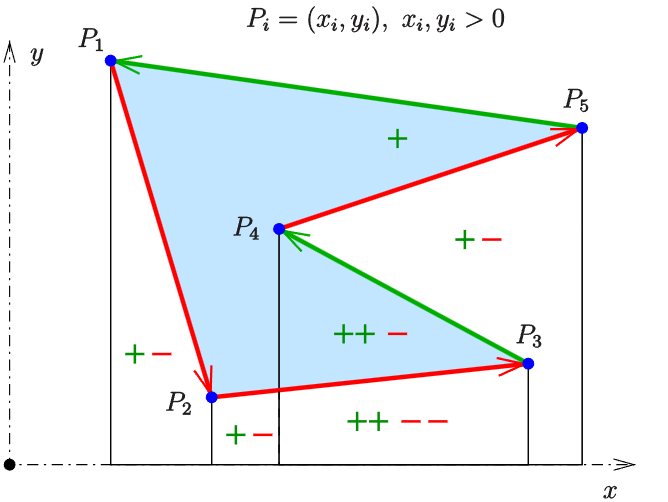
\includegraphics[width=8cm]{bachelors-thesis/shoelace.png}
			\caption{
				This figure shows a geometrical interpretation of the shoelace formula. In difference to the proposition, here the vertices are called $P_i$ and not $\vec{v}_i$. \\
				Source: \cite{ShoelaceFigure2022}}
			\label{fig:shoelace}
		\end{center}
	\end{figure}
	\qed
\end{proposition}

With the Shoelace formula we are able to easily compute all cell areas at all times in the simulation. 
This enables us to implement the gradient flow over the area energy. 

\begin{definition} \textbf{Area energy} \\
	The energy $A_{i}$, used to keep the cell $i$ at a constant volume, reads 
	\begin{align}
		A_i(C_i) = \frac{1}{2} | A_i^d - A_{C_i}|^2, \label{eq:areaEnergy} 
	\end{align}
	where $A_i^d$ is the desired cell area of cell $i$ and $A_{C_i}$ is the current cell area. 
	If not stated otherwise, $A_i^d$ is the initial area of the $i$th cell at the start of the simulation. 
\end{definition}

To maintain the cell area during the simulation, we evaluate the gradient flow of the area energy which indicates the direction of motion for each vertex for preserving the cell area.

\begin{proposition} \textbf{Area force} \\
	The gradient of $\nabla_{\vec{v}^{\: i}_j} A_i(C_i)$ with respect to the $j$th vertex of cell $i$ is given by 
	\begin{center}
		$\nabla_{\vec{v}^{\: i}_j} A_i(C_i) = \dfrac{1}{2} (A_{C_i} - A_i^d) \begin{pmatrix} v_{j+1}^{i,2} - v_{j-1}^{i,2} \\[0.5em]  v_{j-1}^{i,1} - v_{j+1}^{i,1} \end{pmatrix}$, 
	\end{center}
	where $\vec{v}^{\: i}_j = (v_{j}^{i,1}, v_{j}^{i,2})^T$. \\

	Thus, the area force that gets applied on $\vec{v}^{\: i}_j$ is given by 
	\begin{align}
		F_{j}^{(A_i)}(C_i) 
		= - \nabla_{\vec{v}^{\: i}_j} A_i(C_i) 
		= \frac{1}{2}(A_i^d - A_{C_i}) \begin{pmatrix} v_{j+1}^{i,2} - v_{j-1}^{i,2} \\[0.5em]  v_{j-1}^{i,1} - v_{j+1}^{i,1} \end{pmatrix}.
	\end{align}



	Proof.\\
	%TODO: check for correct signs 
	For notational convenience, the subscript $i$ is dropped, since the analysis focuses on a single cell.
	Choose $1 \leq j \leq N_V$.  
	Let us first assume that $A^d \geq A_{C}$ to deal with the absolute value in the area energy. 
	Then, we can compute 
 
	\begin{align*}
		\nabla_{\vec{v}_j} A(C) &= \nabla_{\vec{v}_j} \frac{1}{2} | A^d - A_{C} |^2  \\ 
		&=   |A^d - A_{C}| \nabla_{\vec{v}_j} ( A^d - A_{C})  \\
		&=   |A^d - A_{C}| \nabla_{\vec{v}_j} ( - A_{C}) \\ 
		&=   |A^d - A_{C}| \nabla_{\vec{v}_j} ( - \frac{1}{2} \sum\limits_{k = 1}^{N} (v_k^1 v_{k+1}^2 - v_{k+1}^1 v_k^2)) \\[0.5em]  
		&=   - \frac{1}{2} |A^d - A_{C}| \begin{pmatrix}
			\partial_{v_j^1} (v_j^1 v_{j+1}^2 - v_j^1 v_{j-1}^2)  \\[0.5em]
			\partial_{v_j^2} (v_{j-1}^1 v_j^2 - v_{j+1}^1 v_j^2)
		\end{pmatrix} \\[0.5em] 
		&=   - \frac{1}{2} |A^d - A_{C}| \begin{pmatrix}
			  v_{j+1}^2 - v_{j-1}^2  \\
			 v_{j-1}^1  - v_{j+1}^1 
		\end{pmatrix} 
	\end{align*}

	Remember that $A^d$ is just an independent constant. 
	In the other case, where $A^d < A_{C}$, there is just a change in the sign. 
	Overall, we can write 
\begin{center}
	$
	\nabla_{\vec{v}_j} A(C) = - \frac{1}{2} (A^d - A_{C}) \begin{pmatrix}
		v_{j+1}^2 - v_{j-1}^2  \\[0.5em]
	   v_{j-1}^1  - v_{j+1}^1 
  	\end{pmatrix}.
	$
\end{center}

	\qed
\end{proposition}
It is also valid to write $F_{j}^{(A_i)}(\vec{C})$ instead of $F_{j}^{(A_i)}(C_i)$, since $C_i$ is included in $\vec{C}$. 




    
\subsection{Edge force}
The next force we would like to model is the edge force. 
It acts on the cell's edges and aims to maintain their lengths.


\subsection{Interior angle force}

\subsection{Overlap force}
% explain the algorithm

\subsection{A simulation run}
% state the force system
% DifferentialEquations.jl solver \\
%  -> Euler Maruyama method with fixed time step size  \\